\documentclass[t]{beamer}
\usepackage{helvet}
\usepackage{calc}
\usepackage[utf8]{inputenc}
\usepackage[english]{babel}

\usetheme{Ilmenau}

\setbeamercovered{transparent}
\setbeamertemplate{navigation symbols}{}

\usepackage{units}
\usepackage{amsbsy}
\usepackage{amsmath}
\usepackage{amssymb}
\usepackage{graphics}
\usepackage{graphicx}
\usepackage{epsf}
\usepackage{epsfig}
\usepackage{fixmath}
%\usepackage{pgfmath}
\usepackage{wrapfig}


\title{Quo vadis, Prometheus?}
\subtitle{Monitoring at scale}
\author{Richard Hartmann,\\
RichiH@\{freenode,OFTC,IRCnet\},\\
richih@\{fosdem,debian,richih\}.org,\\
richard.hartmann@space.net}
\date{2017-11-15}


\begin{document}

% hide all subsections
\setcounter{tocdepth}{1}

\section{Introduction}

\subsection{}

\begin{frame}
	\titlepage
\end{frame}

%\begin{frame}
%	\frametitle{Statistics}
%	\tableofcontents
%\end{frame}

\subsection{}

\begin{frame}
	\frametitle{`whoami`}
	\begin{itemize}
%		\item Richard "RichiH" Hartmann
		\item Swiss army chainsaw at SpaceNet
		\item FOSDEM, DebConf, DENOGx, PromCon staff
		\item Author of \url{https://github.com/RichiH/vcsh}
		\item Debian Developer
		\item Prometheus team member
		\item Currently responsible for building one of the most modern datacenters in Europe
		\item ...and always looking for nice co-workers in the Munich area
	\end{itemize}
\end{frame}


\section{Quick intro}

\subsection{Do we even need this section?}

% API commitments
% one exporter per service
% focus on services
% failures happen at scale

% HA? run two
% federation
% kein auth/encryption -> reverse proxy


\begin{frame}
	\frametitle{Show of hands}
	\begin{itemize}
		\item Who has heard of Prometheus?
		\item Who is considering to use Prometheus?
		\item Who is POCing Prometheus?
		\item Who uses Prometheus in production?
	\end{itemize}
\end{frame}

\begin{frame}
	\frametitle{Prometheus 101}
	\begin{itemize}
		\item Inspired by Google's Borgmon
		\item Time series database
		\item float64 timestamp, float64 value
		\item Instrumentation \& exporters
		\item Not for event logging
		\item Dashboarding via Grafana
	\end{itemize}
\end{frame}

\begin{frame}
	\frametitle{Main selling points}
	\begin{itemize}
		\item Highly dynamic, built-in service discovery
		\item No hierarchical model, n-dimensional label set
		\item PromQL: for processing, graphing, alerting, and export
		\item Simple operation
		\item Highly efficient
	\end{itemize}
\end{frame}

\begin{frame}
	\frametitle{Cloudy with a chance of buzzwords}
	\begin{itemize}
		\item So it's built with highly dynamic environments in mind
		\item Containers, sidecars, microservices, ALL the cloud
		\item But it's a monolithic application
		\vfill
		\item ...why?
	\end{itemize}
\end{frame}

\begin{frame}
	\frametitle{Resilience, resilience, and also resilience}
	\begin{itemize}
		\item What do you need for operations?
		\item Power and cooling
		\item Network connectivity
		\item Monitoring
		\item The rest you can fix
	\end{itemize}
\end{frame}


\section{New features in 2.0}
\subsection{}

\begin{frame}
	\frametitle{All new and shiny 2.0}
	\begin{itemize}
		\item Released on 2017-11-08
		\begin{itemize}
			\item (Yes, I did suggest we release today along with this talk)
		\end{itemize}
		\item Various cleanups and improvements
		\item See \url{https://github.com/prometheus/prometheus/releases}
	\end{itemize}
\end{frame}

\begin{frame}
	\frametitle{Three main features}
	\begin{itemize}
		\item Storage backend
		\begin{itemize}
			\item Caveat: Prometheus 2.0 comes with storage v3
		\end{itemize}
		\item Staleness handling
		\item Remote read \& write API is now stable
		\item Links to in-depth talks about these features are at the end of these slides
	\end{itemize}
\end{frame}


\subsection{Storage}

\begin{frame}
	\frametitle{Prometheus 1.x}
	\begin{itemize}
		\item We used to have one file per time series
		\item Easy to implement
		\begin{itemize}
			\item Look up label set
			\item Map files directly to RAM
			\item Let the OS figure out caching etc
			\item Use data
		\end{itemize}
		\item Why change?
	\end{itemize}
\end{frame}

\begin{frame}
	\frametitle{Churn}
	\begin{itemize}
		\item Churn was becoming more and more of a problem
		\item There's a company with a 15 minute maximum lifetime for their containers
		\item If you have a lot of files which might contain data for any given time frame, you need to look at all of them
	\end{itemize}
\end{frame}

\begin{frame}
	\frametitle{Storage v3}
	\begin{itemize}
		\item Fabian Reinartz had an idea about new storage
		\item This POC turned out to be so good, we decided to cut a major release for it
		\item How does it work?
	\end{itemize}
\end{frame}

\begin{frame}
	\frametitle{One file per series}
	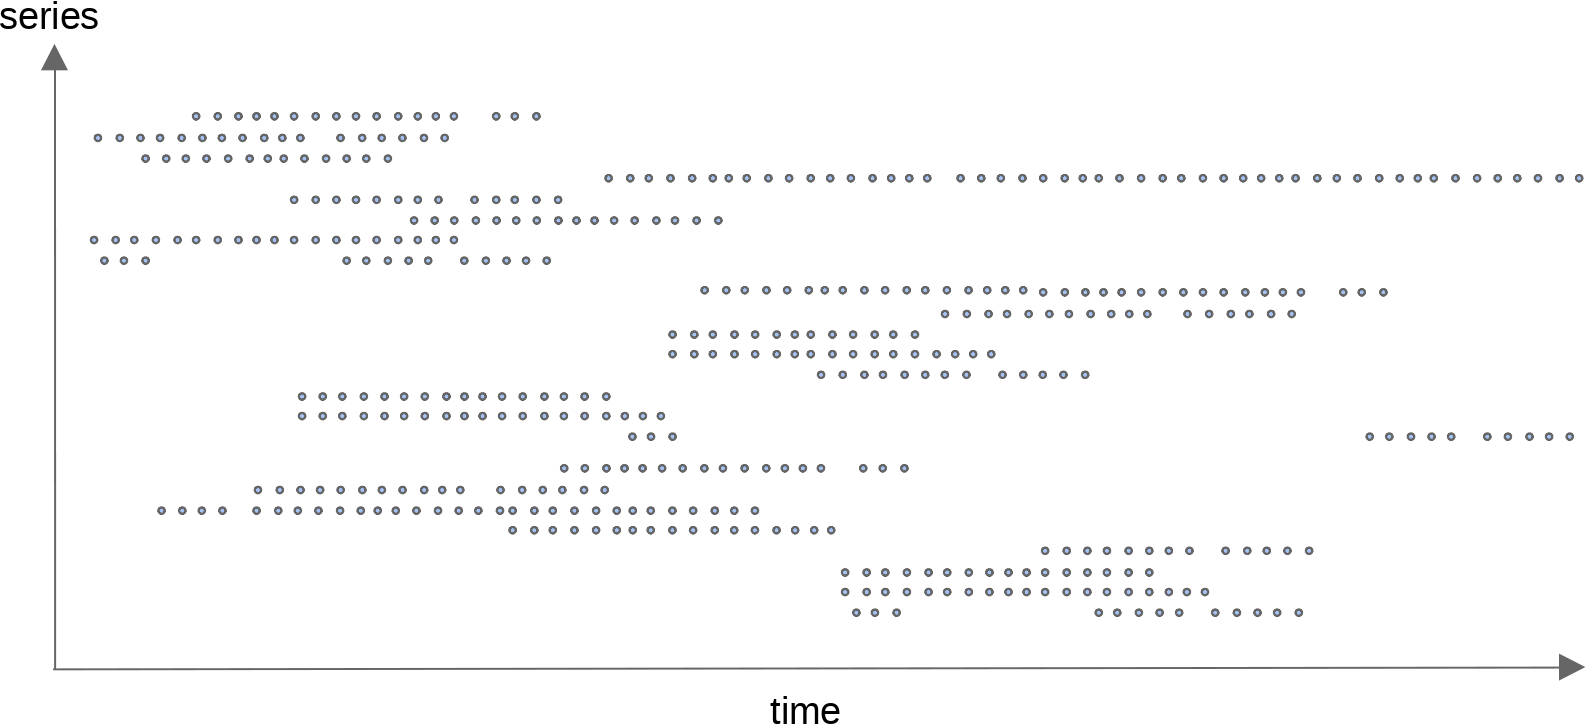
\includegraphics[width=\textwidth]{storage--file_per_series.png}
\end{frame}

\begin{frame}
	\frametitle{Selection}
	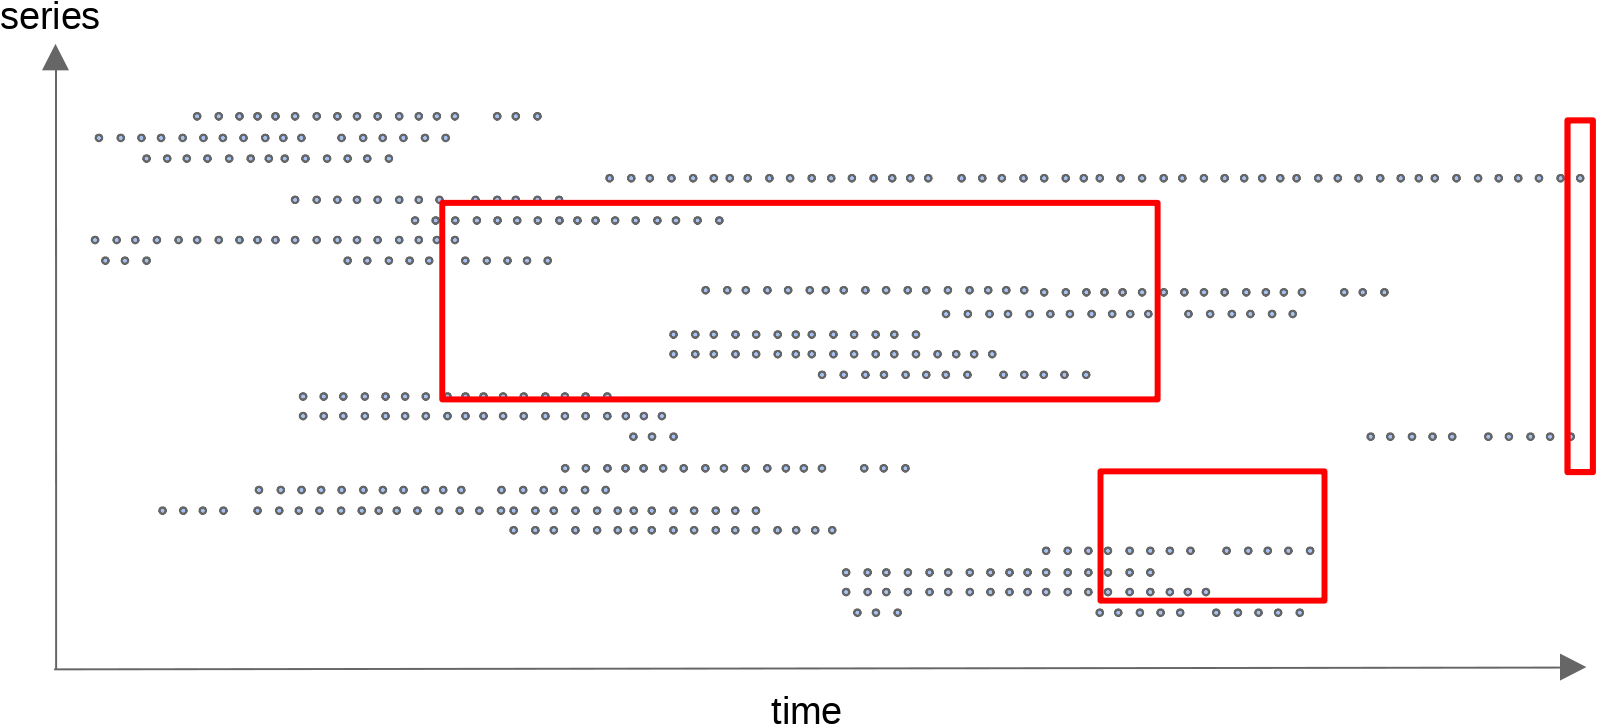
\includegraphics[width=\textwidth]{storage--file_per_series_with_selection.png}
\end{frame}

\begin{frame}
	\frametitle{Blocks}
	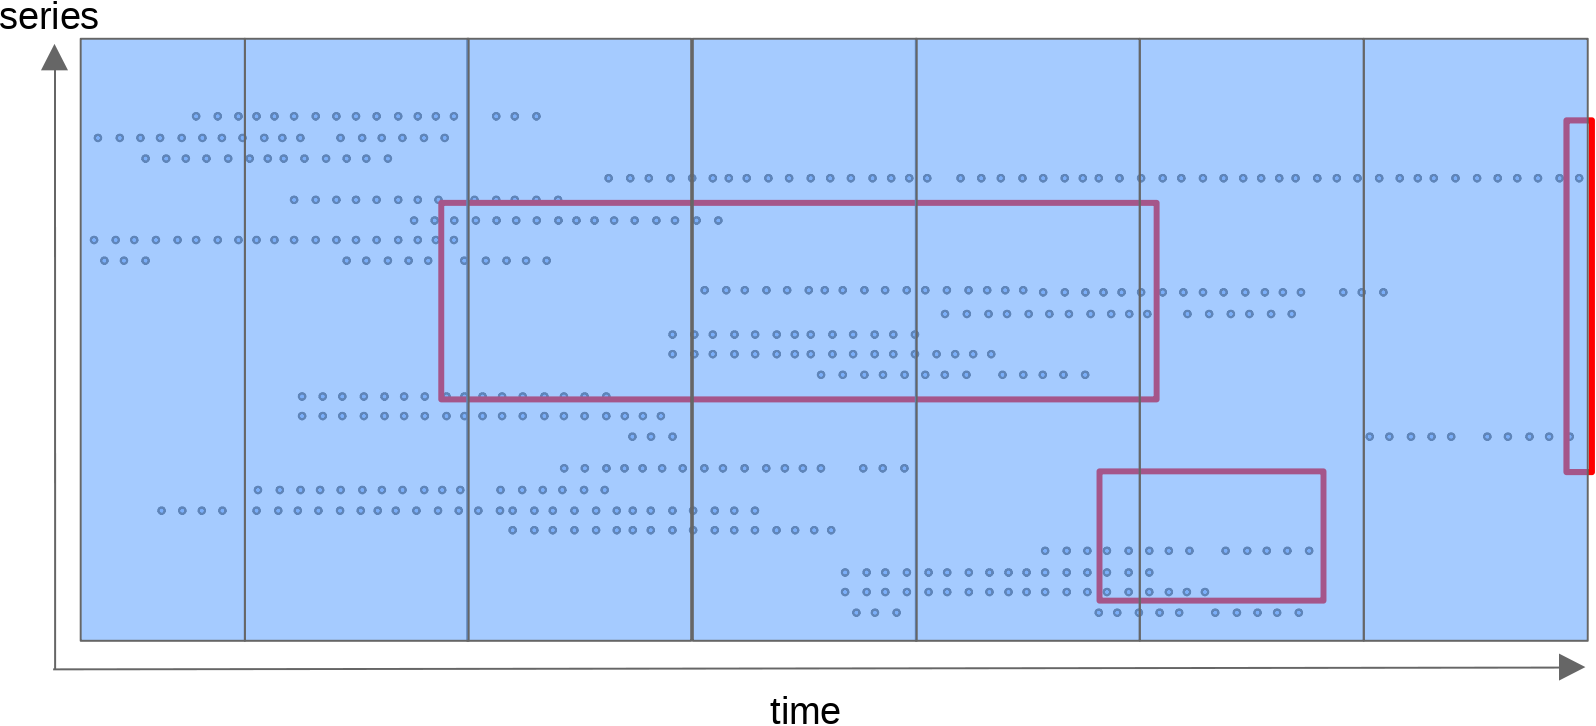
\includegraphics[width=\textwidth]{storage--block_with_selection.png}
\end{frame}

\begin{frame}
	\frametitle{Test setup}
	\begin{itemize}
		\item Kubernetes cluster with dedicated Prometheus nodes
		\item 800 microservice instances and Kubernetes components
		\item 120k samples/sec
		\item 300k active time series
		\item Swap out 50\% of all pods every 10 minutes
	\end{itemize}
\end{frame}

\begin{frame}
	\frametitle{Results}
	\begin{itemize}
		\item 15x reduction in memory usage
		\item 6x reduction in CPU usage
		\item 80-100x reduction in disk writes
		\item 5x reduction in on-disk size
		\item 4x reduction in query latency on expensive queries
	\end{itemize}
\end{frame}

\begin{frame}
	\frametitle{One more thing...}
	\vfill
	Also, you can now properly snapshot and backup Prometheus.
	\vfill
\end{frame}


\subsection{Staleness}


\begin{frame}
	\frametitle{Downside of handling churn}
	\begin{itemize}
		\item So now we can handle extreme churn
		\item ...and suddenly, five minutes staleness timeouts seem awfully long
		\begin{itemize}
			\item Down alerts continue to fire
			\item Double counting
			\item Other icky corner cases
		\end{itemize}
		\item ...and what if you need more than five minutes scrape interval?
	\end{itemize}
\end{frame}

\begin{frame}
	\frametitle{Results}
	\begin{itemize}
		\item When a target goes away, its time series are considered stale
		\item When a target no longer returns a time series, it is considered stale
		\item Longer eval/scrape intervals are now easier to handle
	\end{itemize}
\end{frame}

\begin{frame}
	\frametitle{The way there}
	\begin{itemize}
		\item The actual technical background is too complex for this talk
		\item Find recording and slides by Brian Brazil at the end of this talk
	\end{itemize}
\end{frame}


\subsection{Remote read API}

\begin{frame}
	\frametitle{Playing nicely with others}
	\begin{itemize}
		\item We now have a stable remote read/write API
		\item Which we're already using ourselves; it's the recommended upgrade path from 1.x
		\item You need to upgrade to 1.8.2 to get the correct version in 1.x
	\end{itemize}
\end{frame}


\subsection{Downsides..}

\begin{frame}
	\frametitle{So, about backfill and explicit timestamps...}
	\begin{itemize}
		\item If explicit timestamps were icky before, this has now become worse
		\item You can not ingest data older than the age of the current storage block, nor data much newer
		\item Staleness vs timestamps is non-trivial
	\end{itemize}
\end{frame}



\section{Onwards!}


\subsection{Prometheus 2.1}

\begin{frame}
	\frametitle{ACID databases...}
	\begin{itemize}
		\item A tomicity - we have that
		\item C onsistency - we have that
		\item I solation - here, there be 2.1 features
		\item D urability - we have that since 2.0
	\end{itemize}
\end{frame}

\begin{frame}
	\frametitle{Isolation}
	\begin{itemize}
		\item Each append action gets a write ID (64 bit monotonic counter)
		\item Every sample's write ID is noted along with value and timestamp
		\item Any append action which has not yet committed or rolled back is ignored at query time
		\item We keep write IDs in memory; if we restart or crash, the atomicity of the write ahead log will protect us
	\end{itemize}
\end{frame}


\subsection{And beyond}

\begin{frame}
	\frametitle{True HA}
	\begin{itemize}
		\item So now all our storage is in self-contained blocks
		\item ...this sounds a lot like objects
		\item There's a working test implementation which uses local disk as a hot cache
		\item ...and pulls the rest of that data from S3
		\item In theory, we could use this to splice data from different Prometheus storages together
	\end{itemize}
\end{frame}

\begin{frame}
	\frametitle{Humble aspirations}
	\begin{itemize}
		\item When we say that we want to change how the world does monitoring, we mean it
		\item One of our most powerful features are labels
		\item Labels are encoded in our exposition format
		\item Some third-party projects and vendors have an issue with supporting a "competing" project
		\item Big shout-out to Paul Dix and InfluxData for adopting Prometheus concepts!
	\end{itemize}
\end{frame}

\begin{frame}
	\frametitle{OpenMetrics}
	\begin{itemize}
		\item We are spinning out Prometheus' exposition format
		\item It will join CNCF as a full project
		\item We will submit an ID and try to get an IETF RFC published
		\item ...so you can sneak this random RFC into the requirements of your next tender ;)
	\end{itemize}
\end{frame}

\begin{frame}
	\frametitle{Already on board}
	\begin{itemize}
		\item Cloudflare
		\item GitLab
		\item Google
		\item Grafana
		\item InfluxData
		\item Kausal.co
		\item Oath.com / Yahoo / Verizon
		\item RobustPerception
		\item SpaceNet
		\item Uber
		\item \url{https://github.com/richih/OpenMetrics}
	\end{itemize}
\end{frame}

\begin{frame}
	\frametitle{PromcCon 2018}
	\begin{itemize}
		\item Current plan is to do it in Munich or Dublin
		\item We will continue to run the conference ourselves, but CNCF is handling money for us
		\item If you want to sponsor a venue, do let us know
		\item We can only accept a venue if a team member is living nearby and is willing to invest the time
	\end{itemize}
\end{frame}

\begin{frame}
	\frametitle{Generally speaking...}
	\begin{itemize}
		\item Yes, we want to change the world
		\item Simple and resilient operation of Prometheus remains a core goal
		\item More project and software integrations... and we're talking to hardware vendors as well
		\item Supporting tomorrow's 10x scale today
	\end{itemize}
\end{frame}



\section{Outro}


\subsection{}


\begin{frame}
	\frametitle{Further reading, and listening}
	\begin{itemize}
		\item Prometheus 2017 Dev Summit: \url{https://docs.google.com/document/d/1DaHFao0saZ3MDt9yuuxLaCQg8WGadO8s44i3cxSARcM/edit}
		\item Storing 16 Bytes at Scale: \url{https://promcon.io/2017-munich/talks/staleness-in-prometheus-2-0/}
		\item Staleness and Isolation in Prometheus 2.0: \url{https://promcon.io/2017-munich/talks/staleness-in-prometheus-2-0/}
		\item OpenMetrics: \url{https://github.com/richih/OpenMetrics}
	\end{itemize}
\end{frame}


\begin{frame}
	\frametitle{Thanks!}
		\begin{center}
			\vfill
			Thanks for listening!\\
			\vfill
			Questions?
			\vfill
			Email me if you want a job in Munich.
			\vfill
			See slide footer for contact info.
			\vfill
		\end{center}
\end{frame}

\end{document}

%\begin{frame}
%	\frametitle{}
%	\begin{itemize}
%		\item 
%		\item 
%		\item 
%		\item 
%		\item 
%	\end{itemize}
%\end{frame}
